\documentclass{whuthesis}

\whusetup
{
    info               =
    {
        title          = {基于GRN的垂体基因表达差异分析},
        student-number = {2017300030039},
        school         = {弘毅学堂},
        author         = {郑晖},
        major          = {计算机科学与技术},
        advisor        = {蔡朝晖, 副教授},
        date           = {2021/04},
        keywords       = {GRN, 系统性神经炎症, 垂体},
        keywords*      = {GRN , systemic neuroinflammation, pituitary},
    },
    style              = 
    {
        bib-file       = {ref/refs},
        graphics-path  = {figs/}
    }
}

\begin{document}
    %% preface
    % abstract
    %% abstract

% abstract-cn
\begin{abstract}
  诸如病毒或细菌感染之类的免疫挑战会引起组织炎症,垂体在炎症事件的调节过程中扮演着重要角色。然而,我们对免疫攻击过程中垂体细胞的转录反应知之甚少。使用基于机器学习与统计学习的生信算法,处理单细胞RNA测序数据,将为我们提供细胞转录反应层级的生物学见解。现在希望运用GRN推断、聚类、基因表达差异分析等算法,对实验科学家收集到的垂体单细胞RNA测序数据进行分析,揭示垂体内部各类细胞在中枢神经内分泌炎症调节过程中的角色以及在该过程中起关键作用的调控因子。

  首先,本文使用基因组学家标注的调控子-目标基因集合训练了一个GRN推断器。依据此模型,本文对实验科学家在小鼠炎症模型上收集到的垂体单细胞转录组数据,进行基因调控网络推断。使用聚类等分析手段对得到的基因调控网络进行处理,推断其细胞种类及状态。然后,统计该聚类标签与处理组标签的匹配度,验证刺激的有效性。最后,依据得到的细胞标签,对不同状态的同一种类垂体细胞分别进行基因表达差异分析,并对不同状态的所有细胞进行GRN矩阵差异分析,探寻免疫攻击过程中垂体细胞的转录反应变化以及驱动这种变化的关键转录因子。

  最终分析结果表明,在垂体各类细胞中,对照组与实验组之间的转录反应都有巨大差异,不同种类垂体细胞都积极参与到炎症调节过程中。但是,不同种类垂体细胞的上调、下调基因集合并不相同,即不同垂体细胞在炎症调节过程中的不同角色。除此之外,本文还鉴定出一类在不同种类垂体细胞中共表达的基因调控子,如Stat、Irf和Nfkb等。

  这项研究的结果扩展了我们对炎症激发过程中垂体单细胞转录反应的了解,并提供了将单细胞RNA测序用于动态功能研究的新思路。
\end{abstract}

% abstract-en
\begin{abstract*}
  Immune challenges such as viral or bacterial infections can cause tissue inflammation, and the pituitary gland plays an important role in the regulation of inflammatory events. However, we know very little about the transcriptional response of pituitary cells during immune attack. Using biosynthesis algorithms based on machine learning and statistical learning to process single-cell RNA sequencing data will provide us with biological insights. Now we hope to use GRN inference, clustering, gene expression differential analysis and other algorithms to analyze the pituitary single-cell RNA sequencing data collected by experimental scientists, and reveal the role of various cells within the pituitary in the regulation of central neuroendocrine inflammation and the regulatory factors.

  First, this article uses the regulator-target gene set annotated by genomicists to train a GRN inference machine. Based on this model, this article uses the pituitary single-cell transcriptome data to infer gene regulatory networks. Then, this article use analysis methods to process the obtained gene regulatory network and infer its cell type and state. Finally, according to the obtained cell label, the gene expression difference analysis of the same type of pituitary cells in different states is performed, and the GRN matrix difference analysis is performed on all cells in different states to explore the transcriptional response changes of pituitary cells during immune attack and the key transcription factors.

  The final analysis results showed that in various types of pituitary cells, there are huge differences in the transcriptional response between the control group and the experimental group, and different types of pituitary cells are actively involved in the process of inflammation regulation. However, different types of pituitary cells have different sets of up- and down-regulated genes, that is, different pituitary cells have different roles in the regulation of inflammation. In addition, this article identified some gene regulators that are co-expressed in different types of pituitary cells, such as Stat, Irf, and Nfkb.

  The results of this study expand our understanding of the pituitary single-cell transcriptional response during inflammation stimulation.
\end{abstract*}



    %% main body
    %% chapter 1

\chapter{绪论}
\section{研究背景}
  在病毒或细菌感染期间,免疫因子会在人体中释放,通常会导致组织发炎并导致严重的疾病行为,例如食欲不振,嗜睡,退出正常的社交活动,疲劳,探索力下降等。人们认为疾病行为是由可溶性促炎性细胞因子(IL-1、$TNF-\alpha$、IL-6等)触发的,该因子由感染部位的免疫细胞产生,并会对神经内分泌系统,特别是下丘脑-垂体-肾上腺(HPA)轴\cite{chrousos1995hypothalamic,shanks2000early}产生深远的影响。

  HPA轴是体内的压力反应中心,连接中枢神经系统(CNS)和内分泌系统,其在炎症状态下的调节过程如\ref{fig:HPA}所示。作为HPA轴组成部分的垂体,在炎症事件调节过程中起到重要的作用。由炎症事件诱导的细胞因子(IL1,IL6,TNF-$\alpha$,IFN-$\gamma$)通常循环至垂体前叶,并主要作用于垂体的促肾上腺皮质激素,从而促进释放抗炎激素,例如肾上腺皮质激素(ACTH)。ACTH被携带到肾上腺并作用于ACTH受体,从而上调肾上腺皮质肾上腺皮质细胞中皮质醇的释放。随后,皮质醇在下丘脑和垂体在HPA轴上产生负反馈,以抑制促炎性细胞因子的进一步合成和释放。此外,卵泡细胞代表垂体前叶中唯一的非内分泌细胞类型,并释放可能潜在影响垂体局部激素产生的IL1和IL6,从而构成调节炎症反应的复杂系统。

\begin{figure}[!htb]
  \centering
  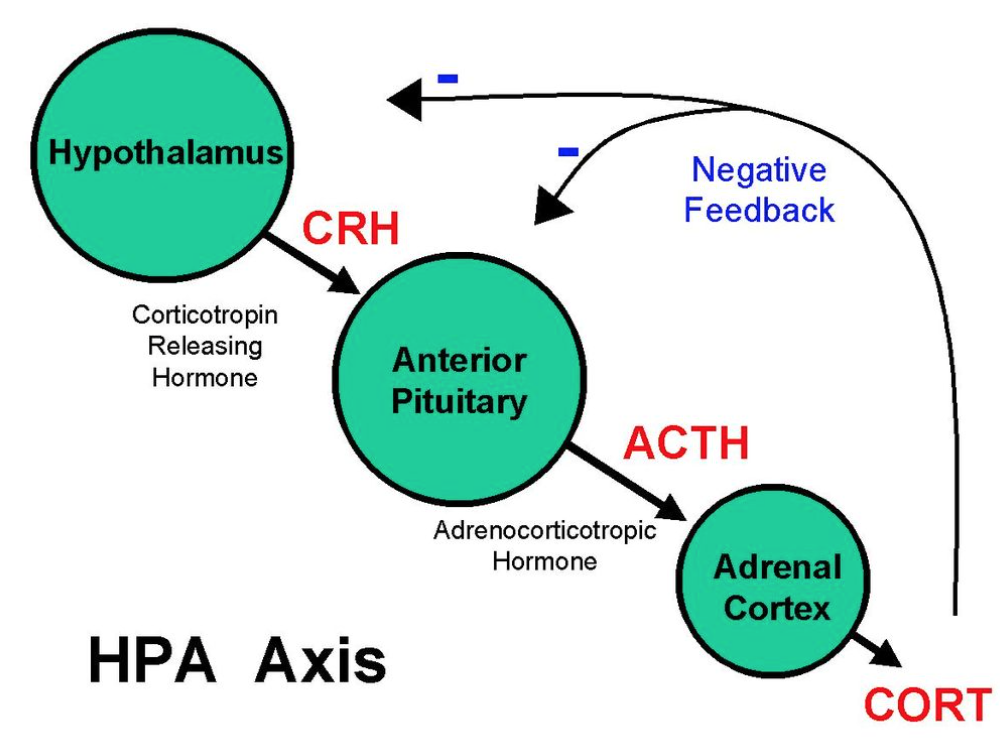
\includegraphics[width=0.6\textwidth]{figs/HPA.png}
  \caption{炎症状态下的HPA轴}
  \label{fig:HPA}
\end{figure}

\section{研究现状与研究内容}
  以往探究垂体在中枢神经内分泌炎症调节过程中作用的研究\cite{chrousos1995hypothalamic,shanks2000early}都没有涉及到单细胞转录层级,没有揭示垂体内部各类细胞在中枢神经内分泌炎症调节过程中的角色以及内在调控因子。

  近几年随着单细胞RNA测序技术的发展\cite{svensson2018exponential},研究人员开始从单细胞转录组水平探究垂体相关的一些问题\cite{chen2020single,cheung2018single,ho2020single,fletcher2019cell},但这些工作主要关注于某个发育过程中的静态分类问题,很少有研究使用单细胞转录组测序来进行动态功能研究。

  这项研究主要关注不同的垂体细胞如何响应炎症刺激。本文使用Seurat\cite{butler2018integrating,stuart2019comprehensive}规定的标准处理流程和基因调控网络推断SCENIC\cite{aibar2017scenic,van2020scalable}算法,对实验科学家收集的垂体单细胞RNA测序数据进行分析,以探究垂体内部各类细胞在中枢神经内分泌炎症调节过程中的角色以及内在调控因子,动态炎症研究将成为这项研究中最重要的部分。这项研究可以使我们对人体对病毒或细菌感染的免疫防御具有更清晰的认识。更重要的是,它具有非常重要的临床意义,我们希望获得用于免疫诊断的特定标记。此外,这项研究也可以为我们提供关于单细胞转录组测序技术应用的新思路。

\section{研究结果}
  在这项研究中,主要贡献有:(1)提供了不同种类垂体细胞参与中枢神经内分泌炎症调节过程的单细胞转录层级证据。(2)揭示了不同种类垂体细胞在参与中枢神经内分泌炎症调节的过程中的转录水平差异,表明其在炎症调节过程中扮演不同的角色。(3)发现了一类在不同种类垂体细胞中统一表达的转录因子,表明其在垂体参与中枢神经内分泌炎症调节过程中的重要地位。

  文章结构安排如下:第二章介绍单细胞测序以及基因调控网络(GRN)的相关工作;第三章介绍单细胞RNA测序数据处理流程;第四章介绍SCENIC算法原理及优势;第五章介绍使用GRN对小鼠垂体单细胞测序数据进行分析;第六章总结了该项工作的结论并对未来的工作进行了展望。


    %% chapter 2

\chapter{公式插图表格}
\section{公式的使用}
在文中引用公式可以这么写:\(a^2 + b^2 = c^2\)。这是勾股定理,它还可以表示为 \(c = \sqrt{a^2 + b^2}\)。还可以让公式单独一段并且加上编号:
\begin{equation}
  \sin^2{\theta} + \cos^2{\theta} = 1 \label{eq:pingfanghe}
\end{equation}
注意,公式前请不要空行。

还可以通过添加标签在正文中引用公式,如式\eqref{eq:pingfanghe}。

我们还可以轻松打出一个漂亮的矩阵:
\begin{equation}
  \vb*{A} =
  \begin{bmatrix}
    1  & 2  & 3  & 4  \\
    11 & 22 & 33 & 44 \\
  \end{bmatrix} \times
  \begin{bmatrix}
    22 & 24 \\
    32 & 34 \\
    42 & 44 \\
    52 & 54 \\
  \end{bmatrix}
\end{equation}

或者多行对齐的公式:
\begin{equation}
  \begin{aligned}
    f_1(x) & = (x + y)^2         \\
           & = x^2 + 2 x y + y^2
  \end{aligned}
\end{equation}

模板使用了 unicode-math 包更改数学字体。所以在使用数学字体时,尽量使用 unicode-math 包提供的 \verb|\sym| 接口,详情请阅读 unicode-math 文档。

\section{插图的使用}
\LaTeX{} 环境下可以使用常见的图片格式:JPEG、PNG、PDF 等。当然也可以使用 \LaTeX{} 直接绘制矢量图形,可以参考 pgf/ti\emph{k}z 等包中的相关内容。需要注意的是,无论采用什么方式绘制图形,首先考虑的是图片的清晰程度以及图片的可理解性,过于不清晰的图片将可能会浪费很多时间。

\begin{figure}[!htb]
  \centering
  
\includegraphics[width=0.3\textwidth]{logo/whulogo.pdf}
  \caption{插图示例}
  \label{fig:whu}
\end{figure}

\verb|[htbp]| 选项分别是此处、页顶、页底、独立一页。\verb|[width=\textwidth]| 让图片占满整行,或 \verb|[width=2cm]| 直接设置宽度。可以随时在文中进行引用,如图~\ref{fig:whu},建议缩放时保持图像的宽高比不变。

\section{表格的使用}
表格的输入可能会比较麻烦,可以使用在线的工具,如 \href{https://www.tablesgenerator.com/}{Tables Generator} 能便捷地创建表格,也可以使用离线的工具,如 \href{https://ctan.org/pkg/excel2latex}{Excel2LaTeX} 支持从 Excel 表格转换成 \LaTeX{} 表格。\href{https://en.wikibooks.org/wiki/LaTeX/Tables}{LaTeX/Tables} 上及 \href{https://www.tug.org/pracjourn/2007-1/mori/mori.pdf}{Tables in LaTeX} 也有更多的示例能够参考。

\subsection{普通表格}
下面是一些普通表格的示例:

\begin{table}[ht]
  \centering
  \caption{简单表格}
  \label{tab:1}
  \begin{tabular}{|l|c|r|}
    \hline
    我是 & 一只 & 普通 \\
    \hline
    的   & 表格 & 呀   \\
    \hline
  \end{tabular}
\end{table}

也可以使用 booktabs 包创建三线表。

\begin{table}[ht]
  \centering
  \caption{一般三线表}
  \label{tab:2}
  \begin{tabular}{ccc}
    \toprule
    姓名 & 学号 & 性别 \\
    \midrule
    张三 & 001  & 男   \\
    李四 & 002  & 女   \\
    \bottomrule
  \end{tabular}
\end{table}

三线表中三条横线分别使用 \verb|\toprule|、\verb|\midrule| 与 \verb|\bottomrule|。另可使用 \verb|\cmidrule{m-n}| 添加 \(m\)--\(n\) 列的横线线。

要创建占满给定宽度的表格需要使用到 tabularx 包提供的 tabularx 环境。引用表格与其它引用一样,只需要表~\ref{tab:3}。

\begin{table}[ht]
  \centering
  \caption{占满文字宽度的三线表}
  \label{tab:3}
  \begin{tabularx}{\textwidth}{CCCC}
    \toprule
    序号 & 年龄 & 身高   & 体重  \\
    \midrule
    1    & 14   & 156    & 42    \\
    2    & 16   & 158    & 45    \\
    3    & 14   & 162    & 48    \\
    4    & 15   & 163    & 50    \\
    \cmidrule{2-4} %添加2-4列的中线
    平均 & 15   & 159.75 & 46.25 \\
    \bottomrule
  \end{tabularx}
\end{table}

\subsection{跨页表格}
跨页表格常用于附录(把正文懒得放下的实验数据统统放在附录的表中)。一般使用 longtable 包提供的 longtable 环境。若要要创建占满给定宽度的跨页表格,可以使用 xltabular 包提供的 xltabular 环境,使用方法与 longtable 类似。以下是一个文字宽度的跨页表格的示例:

\begin{xltabular}{\textwidth}{CCCCCCCCC}
  \caption{文字宽度的跨页表格示例}  \\
  \toprule
  1 & 0 & 5 & 1 & 2 & 3 & 4 & 5 & 6 \\
  \midrule
  \endfirsthead

  \multicolumn{9}{l}{接上一页}      \\
  \toprule
  1 & 0 & 5 & 1 & 2 & 3 & 4 & 5 & 6 \\
  \midrule
  \endhead

  \toprule
  \multicolumn{9}{r}{转下一页}
  \endfoot

  \bottomrule
  \endlastfoot

  1 & 0 & 5 & 1 & 2 & 3 & 4 & 5 & 6 \\
  1 & 0 & 5 & 1 & 2 & 3 & 4 & 5 & 6 \\
  1 & 0 & 5 & 1 & 2 & 3 & 4 & 5 & 6 \\
  1 & 0 & 5 & 1 & 2 & 3 & 4 & 5 & 6 \\
  1 & 0 & 5 & 1 & 2 & 3 & 4 & 5 & 6 \\
  1 & 0 & 5 & 1 & 2 & 3 & 4 & 5 & 6 \\
  1 & 0 & 5 & 1 & 2 & 3 & 4 & 5 & 6 \\
  1 & 0 & 5 & 1 & 2 & 3 & 4 & 5 & 6 \\
  1 & 0 & 5 & 1 & 2 & 3 & 4 & 5 & 6 \\
  1 & 0 & 5 & 1 & 2 & 3 & 4 & 5 & 6 \\
  1 & 0 & 5 & 1 & 2 & 3 & 4 & 5 & 6 \\
  1 & 0 & 5 & 1 & 2 & 3 & 4 & 5 & 6 \\
  1 & 0 & 5 & 1 & 2 & 3 & 4 & 5 & 6 \\
  1 & 0 & 5 & 1 & 2 & 3 & 4 & 5 & 6 \\
  1 & 0 & 5 & 1 & 2 & 3 & 4 & 5 & 6 \\
  1 & 0 & 5 & 1 & 2 & 3 & 4 & 5 & 6 \\
  1 & 0 & 5 & 1 & 2 & 3 & 4 & 5 & 6 \\
  1 & 0 & 5 & 1 & 2 & 3 & 4 & 5 & 6 \\
  1 & 0 & 5 & 1 & 2 & 3 & 4 & 5 & 6 \\
  1 & 0 & 5 & 1 & 2 & 3 & 4 & 5 & 6 \\
  1 & 0 & 5 & 1 & 2 & 3 & 4 & 5 & 6 \\
  1 & 0 & 5 & 1 & 2 & 3 & 4 & 5 & 6 \\
  1 & 0 & 5 & 1 & 2 & 3 & 4 & 5 & 6 \\
  1 & 0 & 5 & 1 & 2 & 3 & 4 & 5 & 6 \\
  1 & 0 & 5 & 1 & 2 & 3 & 4 & 5 & 6 \\
  1 & 0 & 5 & 1 & 2 & 3 & 4 & 5 & 6 \\
  1 & 0 & 5 & 1 & 2 & 3 & 4 & 5 & 6 \\
  1 & 0 & 5 & 1 & 2 & 3 & 4 & 5 & 6 \\
  1 & 0 & 5 & 1 & 2 & 3 & 4 & 5 & 6 \\
  1 & 0 & 5 & 1 & 2 & 3 & 4 & 5 & 6 \\
  1 & 0 & 5 & 1 & 2 & 3 & 4 & 5 & 6 \\
  1 & 0 & 5 & 1 & 2 & 3 & 4 & 5 & 6 \\
  1 & 0 & 5 & 1 & 2 & 3 & 4 & 5 & 6 \\
  1 & 0 & 5 & 1 & 2 & 3 & 4 & 5 & 6 \\
  1 & 0 & 5 & 1 & 2 & 3 & 4 & 5 & 6 \\
  1 & 0 & 5 & 1 & 2 & 3 & 4 & 5 & 6 \\
\end{xltabular}


\section{列表的使用}
下面演示了创建有序及无序列表,如需其它样式,\href{https://www.latex-tutorial.com/tutorials/lists/}{LaTeX Lists} 上有更多的示例。

\subsection{有序列表}
这是一个计数的列表
\begin{enumerate}
  \item 第一项
        \begin{enumerate}
          \item 第一项中的第一项
          \item 第一项中的第二项
        \end{enumerate}
  \item 第二项
        \begin{enumerate}[label=(\roman*)]
          \item 第一项中的第一项
          \item 第一项中的第二项
        \end{enumerate}
  \item 第三项
\end{enumerate}

\subsection{不计数列表}
这是一个不计数的列表
\begin{itemize}
  \item 第一项
        \begin{itemize}
          \item 第一项中的第一项
          \item 第一项中的第二项
        \end{itemize}
  \item 第二项
  \item 第三项
\end{itemize}

\section{数学环境的使用}
模板简单定义了 8 种数学环境,具体见表~\ref{tab:数学环境},使用方法如下所示。

\begin{table}
  \caption{模板定义的数学环境}\label{tab:数学环境}
  \begin{tabularx}{\textwidth}{CCCC}
    \toprule
    theorem     & definition & lemma  & corollary \\
    定理        & 定义       & 引理   & 推论      \\
    \midrule
    proposition & example    & remark & proof     \\
    性质        & 例         & 注     & 证明      \\
    \bottomrule
  \end{tabularx}
\end{table}

\begin{theorem}
  设向量 \(\vb*{a} \neq \vb*{0}\),那么向量 \(\vb*{b} \parallel \vb*{a}\) 的充分必要条件是:存在唯一的实数 \(\lambda\),使 \(\vb*{b} = \lambda \vb*{a}\)。
\end{theorem}
\begin{definition}
  这是一条定义。
\end{definition}
\begin{lemma}
  这是一条引理。
\end{lemma}
\begin{corollary}
  对数轴上任意一点 \(P\),轴上有向线段 \(\overrightarrow{OP}\) 都可唯一地表示为点 \(P\) 的坐标与轴上单位向量 \(\vb*{e}_u\) 的乘积:\(\overrightarrow{OP} = u \vb*{e}_u\)。
\end{corollary}
\begin{proposition}
  这是一条性质。
\end{proposition}
\begin{example}
  这是一条例。
\end{example}
\begin{remark}
  这是一条注。
\end{remark}
\begin{proof}
  留作练习。
\end{proof}

若要定义自己的数学环境,可通过如下代码实现:
\begin{verbatim}
\newtheorem{nonsense}{胡说}
\newtheorem*{bullshit}{八道}
\end{verbatim}
其中,带星号 * 的命令不会自动编号。

\newtheorem{nonsense}{胡说}
\newtheorem*{bullshit}{八道}

\begin{nonsense}
  啊吧啊吧啊吧。
\end{nonsense}

\begin{bullshit}
  不啦不啦不啦。
\end{bullshit}


    %% chapter 3

\chapter{单细胞RNA测序数据处理流程}

\section{将原始测序数据转化为基因表达矩阵}
  在将生物样品进行测序后,我们会得到内含测序数据的fastq文件。但fastq文件是由高通量测序产生的输出文件,我们不能直接使用它进行数据挖掘。在这项研究中我们使用CellRanger将其转化为基因表达矩阵,并基于此开展下游分析。

  CellRanger是一组分析管道,用于处理Chromium单细胞数据以对齐读取、生成Feature-Barcode矩阵、执行聚类和其他辅助分析等。CellRanger有四个处理管线与3'单细胞基因表达解决方案及其相关产品有关,我们在这里只关注常用的cellranger mkfastq与cellranger count,其对应流程如图\ref{fig:cellranger-workflow}所示。cellranger mkfastq的主要作用是将Illumina测序生成的原始碱基检出(BCL)文件转化为fastq文件。cellranger count对cellranger mkfastq获取的fastq文件执行对齐、过滤、Barcode计数以及UMI计数,我们使用其产生的计数矩阵进行下游分析。

\begin{figure}[!htb]
  \centering
  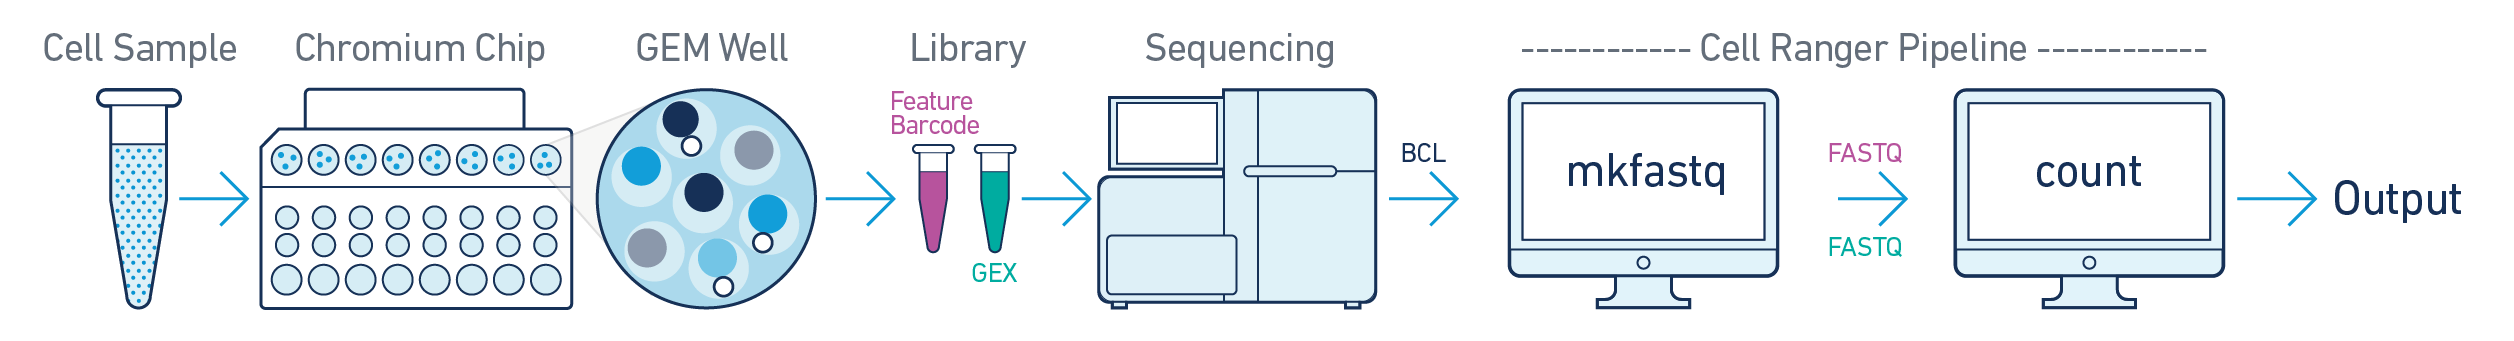
\includegraphics[width=0.8\textwidth]{figs/cellranger-workflow.png}
  \caption{CellRanger工作流程}
  \label{fig:cellranger-workflow}
\end{figure}

\section{对基因表达矩阵进行质量控制}
  对基因表达矩阵进行质控的主要目的是去除制备生物样品和单细胞RNA测序过程中引入的噪音。例如,在进行单细胞RNA测序的过程中,受限于测序芯片的技术条件,会有一定比例将两个细胞吹到同一个测序单位中,又或是使细胞破损等。为了保证下游分析结果的正确性,我们必须将这些离群点检测出来并将其去除。

  目前进行质量控制的主流方法还是阈值法,即对基因表达矩阵在细胞水平(Cell-level QC)、基因水平(Feature-level QC)以及变量水平(Variable-level QC)依据所处理生物数据特性人为设置生物合理的阈值。正常情况下,所检测到的线粒体RNA占所检测到RNA总量的5\%以下,如果高于这个值便可能是在测序的过程中出现细胞破损,导致细胞质RNA外流。但是这种情况也不是绝对的,比如在肌肉细胞中代谢旺盛,所检测到的线粒体RNA占比便会高于此值,因此我们需要针对组织的特异性设定不同的阈值。

  在质量控制之后,我们还可以去除一些已知功能且与研究不相关的RNA(比如核糖体RNA、线粒体RNA),以避免其对下游分析的影响。

\section{依据基因表达矩阵进行聚类}
  在对基因表达矩阵进行质量控制之后,为探求单细胞层级的异质性,我们可以依照其基因表达的差异将其聚类为不同的簇,并鉴定不同簇上的基因marker,为之后的分析提供基础的生物见解。Seurat v3\cite{butler2018integrating,stuart2019comprehensive}建议的初步处理流程是:归一化、特征选择、放缩、线性降维、构建最短近邻图、Leiden聚类和UMAP可视化。
\subsection{特征选取}
  特征选取是在Feature-Barcode矩阵(或者说Gene-Cell矩阵)中计算每个基因的方差,并对其进行排序,选取其中具有较高方差的基因集合(即,它们在某些细胞中高表达,而在其他细胞中低表达)用于下游线性降维。这里使用一些方差较大基因的原因在于,从信息学的角度来看,方差越大的变量蕴含的信息越多。同时,Brennecke等人在2013年的一项研究\cite{brennecke2013accounting}表明在下游分析中关注这些基因有助于去除技术噪声,以在单细胞数据集中突出显示生物信息。线性降维也是基于此原理,对数据进行进一步的筛选,去除方差较低成分的噪声影响。
\subsection{Leiden聚类算法}
  Leiden聚类\cite{traag2019louvain}是整个初步处理流程的关键一步,其依据线性降维结果构建的最短近邻图挖掘其中的群落结构,其原型是Louvain聚类算法\cite{blondel2008fast}。我们下面会详细介绍Louvain算法的局限以及Leiden算法的改进。

  Louvain算法和Leiden算法都是基于图数据的群落发现算法,其灵感源于modularity的优化。其中,modularity是一个定义在$[-1/2,1]$的比例值,用于度量群落内部边缘相对于群落外部边缘的相对密度。对于加权图,modularity由公式(\ref{equ:graph-modularity})定义:
\begin{equation}
  \label{equ:graph-modularity}
  Q = \frac{1}{2m}\sum_{ij}\left[A_{ij} - \frac{k_{i}k_{j}}{2m}\right]\delta(c_{i},c_{j})
\end{equation}
其中,$A_{ij}$表示节点$i$和$j$之间边的权重,$k_{i}$和$k_{j}$分别是连接到节点$i$和$j$的边的权重之和,$m$是图中所有边缘权重的总和,$c_{i}$和$c_{j}$是节点的群落,$\delta$是Kronecker函数(如果$x=y$,$\delta(x,y)=1$,否则为0)。从理论上优化此值会导致给定网络节点的最佳分组,但这在计算上并不可行。因此使用启发式算法,通过迭代来近似modularity的最大值,Louvain算法和Leiden算法都是属于这种形式。

   在Traag等人2019年的一项工作\cite{traag2019louvain}中,实验证据表明Louvain算法得到的分区中会存在连接不良的群落,甚至内部断开的群落。而且他们证明在使用Louvain算法时,该问题在实践中经常发生。在Louvain算法中存在这样一种情况:一个节点在其旧群落中充当不同部分连接的桥梁,但是却可能在群落更新过程中被移动到另一个群落,从其旧群落中删除这样的节点会断开旧群落的连接。Louvain算法可能假设旧群落的其他节点也会移动到该新群落,但事实并非如此,尽管旧群落已经断开连接,但其他节点仍可以与其群落保持牢固的联系,如图\ref{fig:louvain-prob}所示。

\begin{figure}[!htb]
  \centering
  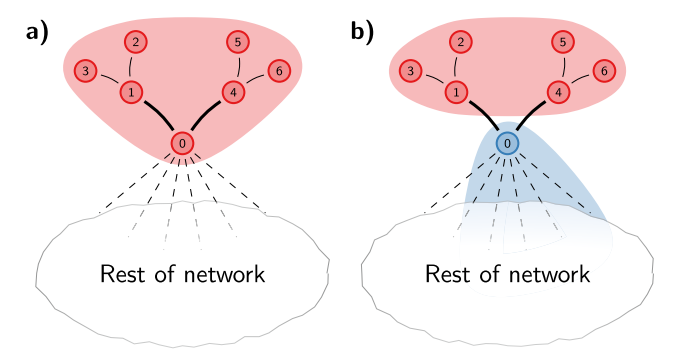
\includegraphics[width=0.8\textwidth]{figs/louvain-prob.png}
  \caption{Louvain算法存在的问题}
  \label{fig:louvain-prob}
\end{figure}

  Leiden算法的改进主要在于利用了加快节点局部移动\cite{ozaki2016simple,bae2017scalable}以及将节点移动到随机邻居\cite{traag2015faster}的思想。Leiden算法由三个阶段组成:(1)节点的局部移动;(2)分区的细化;(3)基于细化的分区进行网络聚合。

  在算法的第一阶段,首先将网络中每个节点分配给其自己对应的群落。然后,对每个节点$i$,计算将其从自身的群落移除并将其移至每个邻居节点$j$对应群落所带来的modularity变化。这两步的公式比较相似,其中将节点$i$移至其邻居节点$j$对应群落所带来modularity的变化由公式(\ref{equ:modularity-change})定义:
\begin{equation}
  \label{equ:modularity-change}
  \Delta{Q} = \left[\frac{{\Sigma}_{in} + 2k_{i,in}}{2m} - \left(\frac{{\Sigma}_{tot} + k_{i}}{2m}\right)^{2}\right] - \left[\frac{{\Sigma}_{in}}{2m} - \left(\frac{{\Sigma}_{tot}}{2m}\right)^{2} - \left(\frac{k_{i}}{2m}\right)^{2}\right]
\end{equation}
其中,${\Sigma}_{in}$是节点$i$将要移入群落中所有连接的权重之和,${\Sigma}_{tot}$是节点$i$将要移入群落中所有连接到节点的权重之和,$k_{i}$是节点$i$的加权度,$k_{in}$是节点$i$与其将要移入群落中所有节点的连接权重之和,$m$是网络中所有连接权重之和。利用加快节点局部移动\cite{ozaki2016simple,bae2017scalable}的思想,仅计算与节点$i$相连所有群落中刚修改群落的modularity,其余沿用以前的计算值。

  在算法的第二阶段产生的分区$\mathcal{P}_{refined}$是Louvain算法对应阶段生成分区$\mathcal{P}$的细分。分区$\mathcal{P}$中的群落可以分为分区$\mathcal{P}_{refined}$中的多个群落。在进行合并的过程中,节点$i$并没有像Louvain算法中那样贪婪地与最大化modularity的群落合并,而是随机选择任何可以增加modularity的群落进行合并。modularity的增加越大,选择该群落的可能性就越大\cite{traag2015faster}。选择群落的随机性允许更广泛的探索分区空间。此外,仅当节点$i$与分区$\mathcal{P}$中的群落充分良好地连接时,才将其与分区$\mathcal{P}_{refined}$中的群落合并,从而避免分区存在连接不良的群落。

  在算法的第三阶段,将第二阶段得到的每一个群落折叠为单个节点,并在此基础上建立新的网络。这时,新群落节点上的自环表示同一群落节点之间的所有连接,而群落节点之间的加权边表示同一群落多个节点到不同群落节点的连接。在新网络创建完毕后,其结果可以重新用于算法的第一阶段,进行迭代,最终得到聚类结果。

  总之,Leiden算法可以保证产生的分区中不会存在连接不良的群落。在Leiden算法被迭代使用时,它会收敛到一个分区,在该分区中,可以确保所有群落的所有子集都属于局部最优分配。因此,Leiden算法可以提供准确的聚类见解,供下游分析使用。


    %% chapter 4

\chapter{实验数据分析}

\section{测序数据预处理}
  通过图\ref{fig:expr-fig1}a所示的流程,我们获取了小鼠垂体细胞的单细胞测序数据。将测序得到的fastq文件利用CellRanger进行上游分析,序列回帖参考基因组选用Ensembl(GRCm38)。回帖得到的基因表达矩阵通过Scater\cite{mccarthy2017scater}进行质量控制,筛除低质量细胞,再用Seurat v3\cite{butler2018integrating,stuart2019comprehensive}进行基础下游分析。

\begin{figure}[!htb]
  \centering
  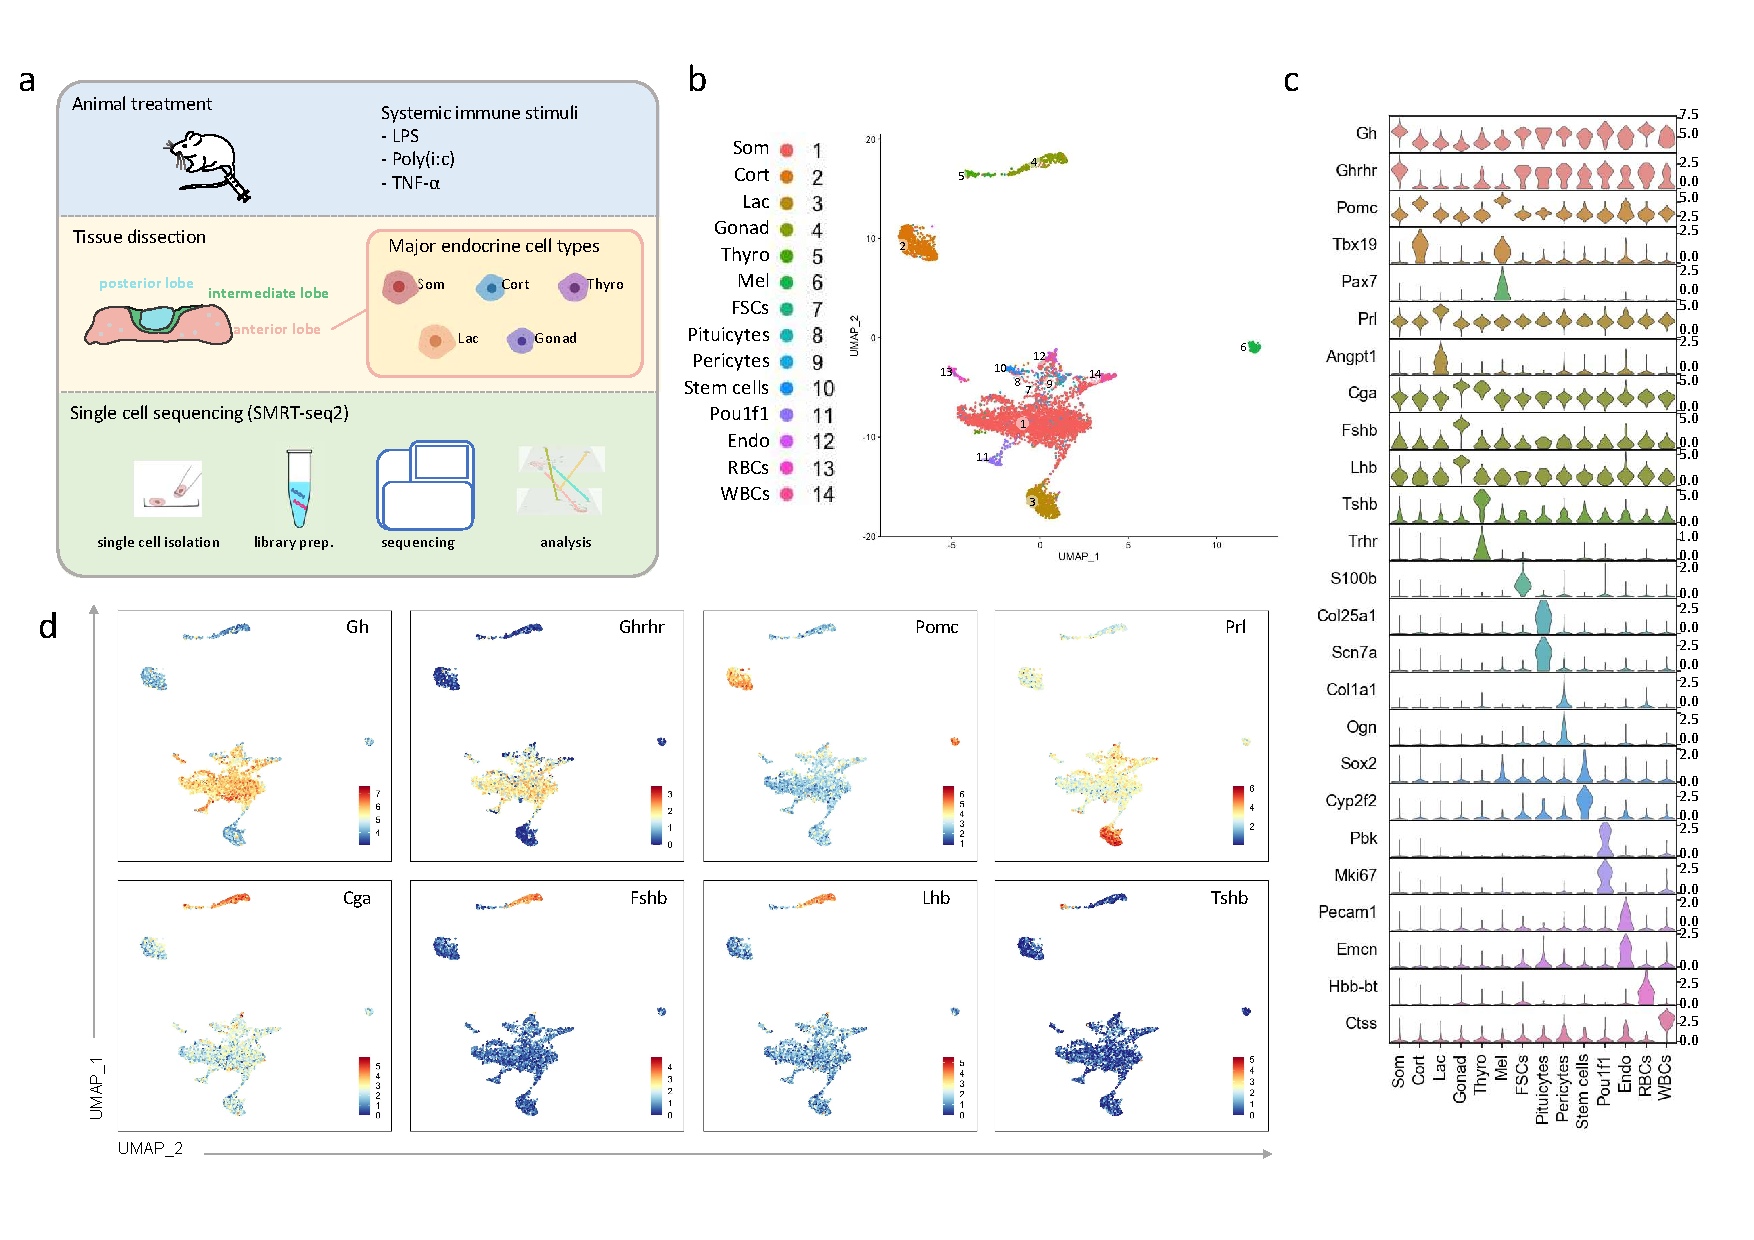
\includegraphics[width=1.0\textwidth]{figs/expr-fig1.pdf}
  \caption{单细胞测序数据预处理}
  \label{fig:expr-fig1}
\end{figure}

\subsection{Scater质控}
  将测序数据读入R工作环境中,将表达矩阵转换为SingleCellExperiment(SCE)对象,对该SCE对象依次在细胞水平(Cell-level QC)、基因水平(Feature-level QC)以及变量水平(Variable-level QC)执行质控。在细胞水平质控中,去除文库含量小(low library size)、基因含量少(low features)和线粒体基因含量高(high mitochondrial percentage)的细胞;在基因水平质控中,去除表达量为0的基因以及线粒体基因、核糖体基因,以避免在PCA部分影响主成分判别;在变量水平中,对每个变量方差解释的贡献率(variance explained)做统计,查看是否有异常变量出现。

  通过STAR-featureCounts上游管线处理后,我们共收集到6727个细胞,平均每个细胞检测到3546个基因。在经过Scater质控后,保留了5506个细胞。
\subsection{Seurat初步分析}
  经过质控处理后的数据转换为Seurat对象,执行Seurat基础分析流程:归一化、特征选择、放缩、线性降维、构建最短临近图、Louvain聚类以及UMAP可视化。

  在此基础上,结合聚类信息以及中枢神经系统各细胞类型已知的基因marker(表\ref{tab:gene-marker}),对数据进行细胞类型注释。我们在垂体腺中鉴定了6个主要细胞簇(Somatotropes,Corticotropes,Melanotropes,Lactotropes,Thyrotropes,Gonadotropes),这与先前的知识是一致的。详见图\ref{fig:expr-fig1}。
\begin{table}[ht]
    \centering
    \caption{中枢神经系统各细胞类型已知的基因marker}
    \label{tab:gene-marker}
    \begin{tabular}{ll}
        \toprule
        细胞类型 & 基因marker \\
        \midrule
        Somatotropes & Gh, Ghrhr, Pappa2, Gnmt \\
        Lactotropes & Prl, Angpt1 \\
        Corticotropes & Pomc, Crhr1, Tbx19 \\
        Melanotropes & Pomc, Tbx19, Pax7, Pcsk2, Rbfox3 \\
        Gonadotropes & Fshb, Lhb, Gnrhr, Cga, Nr5a1 \\
        Thyrotropes & Tshb, Trhr, Cga \\
        Pou1f1 progenitors & Pbk, Top2a, Mki67 \\
        RBCs & Hbb-bt, Hbb-bs \\
        WBCs & C1qa, Ctss, Ptprc \\
        Folliculostellate cells & S100b, Fxyd1 \\
        Endothelial cells & Pecam1, Emcn, Plvap \\
        Pituicytes & Gja1, Scn7a, Col25a1 \\
        Pericytes & Colia1, Dcn, Ogn, Lum, Pdgfrb \\
        Stem cells & Sox2, Aldh3a1, Aldh1a2, Cgp2f2 \\
        \bottomrule
    \end{tabular}
\end{table}

  在这项研究中,我们主要关注的是系统性神经炎症对于垂体细胞的单细胞转录水平影响。因而,我们依据上面得到的细胞注释对数据进行筛选,只留下Somatotropes、Corticotropes、Lactotropes、Thyrotropes以及Gonadotropes五类细胞,共3788个细胞。我们之后的分析便都在此数据上开展。

\section{测序数据SCENIC分析}
  我们对筛选出来的测序数据进行SCENIC分析,以推断其潜在转录因子及对应目的基因。这一步的输出是一个AUC-score矩阵,矩阵的每一个单元表示每一个细胞中对每个基因集合的整体趋势评分,当其符号为正时上调,反之下调。我们对该矩阵进行降维聚类,并用其聚类结果作为细胞是否处于炎症状态的判别标准,如图\ref{fig:expr-fig2}a,b。对于每一类细胞,该分类结果显然可以很好地匹配UMAP可视化后的数据分布。

  在这里,我们使用SCENIC的聚类结果,代替原始基因表达矩阵聚类结果,作为细胞是否处于炎症状态的判别标准。其原因是SCENIC能够觉察到一整个基因集合的整体趋势,去除批次效应所带来的影响,获得更为生物合理的结果。这里所指的批次效应,是由于我们在从多只小鼠上收集数据,会引入一些与生物处理无关的噪声(如温度、研磨程度等),而这些噪声会极大影响基于原始基因表达矩阵的聚类过程。相较之下,SCENIC的结果则可以尽可能降低批次效应所带来的影响。其在GRNBoost之后添加了RcisTarget过程,使得其在推理GRN的时候不再单纯地依赖GRNBoost得到的相关性,而是对GRNBoost推理得到的相关性利用生物学的先验知识进行修剪,只留下具备因果关系的转录因子及其目标基因。

\begin{figure}[!htb]
  \centering
  \includegraphics[width=1.0\textwidth]{figs/expr-fig2.pdf}
  \caption{单细胞测序数据SCENIC分析}
  \label{fig:expr-fig2}
\end{figure}

\subsection{分析处理条件与垂体细胞状态之间的关系}
  在我们所构建小鼠炎症模型中,我们依据免疫刺激剂、给药剂量与恢复时间尺度等因素建立了一系列实验。为了揭示这一系列因素与垂体细胞状态之间的关系,我们将这些处理条件与SCENIC聚类结果进行整合,如图\ref{fig:expr-fig2}c所示。

  我们可以看到所有注射saline的处理组,基本都处于健康(healthy)状态。除此之外,还有注射LPS的处理组也对应到了健康(healthy)状态。通过观察给药剂量与恢复时间尺度因素,我们可以发现这些细胞大多是注射低剂量LPS或者经历了长时程的恢复,在这种情况下神经系统仅有少量垂体细胞处于免疫应激状态。相比之下,注射高剂量LPS且仅经历短时程恢复的处理组则大多处于炎症(inflammation)状态。

\subsection{分析不同细胞在炎症状态下的基因表达差异}
  我们进一步比较了垂体中不同细胞在炎症状态下的基因表达差异,见图\ref{fig:expr-fig2}d。该图的上半部分是垂体各类细胞在其对应基因marker上的基因表达热图。同类细胞对应的基因marker无论中枢神经系统是否处于炎症状态,都会在该类细胞中稳定表达。然后,我们对每一类细胞分析其炎症状态与健康状态下的差异表达基因集合,并将其整合,便得到了该图的下半部分。

  我们发现同处于炎症状态,垂体中不同细胞应对炎症所做出的基因表达调整并不一致。例如,在炎症状态Somatotropes中上调最显著的基因集合并不是在炎症状态Corticotropes中上调最显著的基因集合。这便说明,在中枢神经内分泌系统处于炎症状态时,垂体内各类细胞会采取不同的应激方式,组成一个调节炎症反应的复杂系统。

\subsection{分析导致炎症状态的转录因子}
  我们依据SCENIC过程得到的AUC-score矩阵,统计出每个转录因子的AUC-score密度分布,我们希望找到具备双峰分布或者重尾分布的转录因子。对这些转录因子的分布进行自适应二值化,我们发现其标签可以和之前使用SCENIC聚类结果判定的细胞状态很好地匹配起来(见图\ref{fig:expr-fig3})。

  我们通过上面过程找到的转录因子涉及Stat、Irf以及Nfkb等转录因子家族,这些转录因子大多是与免疫过程相关的。例如,Irf7编码干扰素调节因子7,以往实验数据表明其在病毒诱导的细胞基因(包括I型干扰素基因)的转录中起作用。这些转录因子并没有像之前分析的差异表达基因那样展现出细胞种类特异性,而是在整个炎症状态的垂体细胞中广泛表达。

  这就表明Stat、Irf以及Nfkb等转录因子家族在垂体参与中枢神经内分泌炎症调节过程中扮演着重要的角色,影响着各类垂体细胞的调控路径。换句话说,Stat、Irf以及Nfkb等转录因子家族是垂体参与中枢神经内分泌炎症调节过程中的Master Regulator Genes(MRs)\cite{mattick2010global}。

\begin{figure}[!htb]
  \centering
  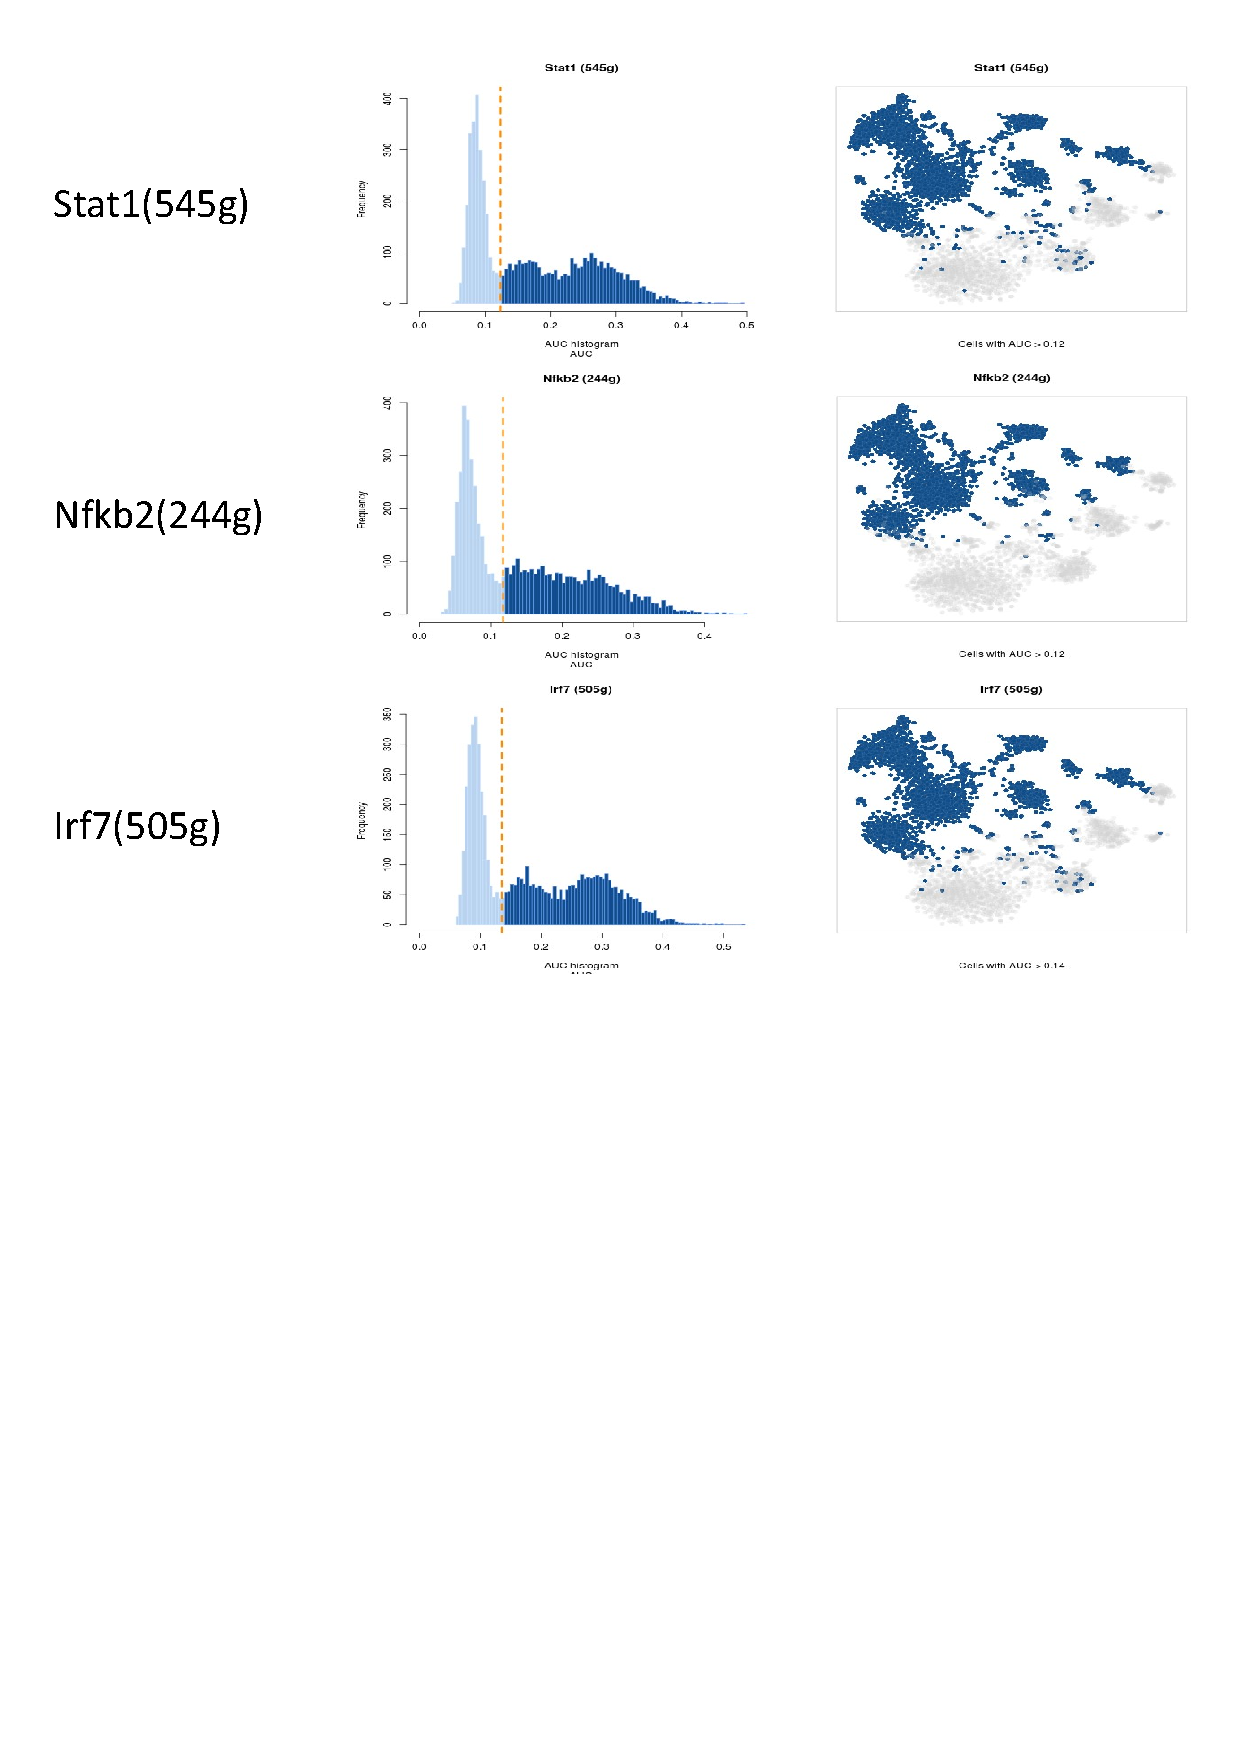
\includegraphics[width=0.8\textwidth]{figs/expr-fig3.pdf}
  \caption{具备双峰分布或者重尾分布的转录因子}
  \label{fig:expr-fig3}
\end{figure}

\section{讨论和未来工作}
  我们在实验中发现,在给以小鼠$TNF-\alpha$刺激之后,其部分垂体细胞在经历UMAP可视化降维之后,呈现出与其他炎症状态细胞相分离的现象。这似乎意味着垂体细胞在参与中枢神经内分泌炎症调节过程中,会因免疫刺激不同而进入不同的调节状态。

  我们初步推断是$TNF-\alpha$作为一种较强的免疫刺激剂,使垂体细胞进入一种不可逆转的免疫状态。在实验设计上,针对LPS、saline与Ploy I:C,我们都设计了长短恢复时程的对比试验,但$TNF-\alpha$只有短时程恢复处理。其原因在于$TNF-\alpha$相比LPS、Ploy I:C产生的免疫反应过于剧烈,小鼠在被腹腔注射500ug$TNF-\alpha$之后无法恢复,6h内便会死亡。

  我们未来的工作便打算在该研究的基础上,进一步探讨面对不可恢复炎症刺激与可恢复炎症刺激时垂体细胞在转录水平上的差异,揭示由健康(healthy)状态向这两种炎症(inflammation)状态转变的关键转录因子。



    %% end
    % ref
    \nocite{*}
    \makebibliography
    % thanks
    %% thanks

\begin{acknowledgements}
  感谢蔡朝晖教授。她是大学期间为我们代课最多的老师,在我大学的学习和成长过程中提供了很大的指导和帮助。大一入学常听陈子轩和原昊博提起蔡老师,经过一段时间的接触,果然对学生十分负责!感谢蔡老师大学四年来对我的信任,让我在计算机本科学习中更加自信。

  感谢北京脑科学与类脑研究中心的罗敏敏教授。他在毕业论文撰写过程中给我提供了很大指导和帮助。我很敬佩罗老师对于科学的近乎狂热般的痴迷与对学生的关心。出于对神经科学的痴迷,我在保研的时候选择放弃我所擅长的计算机系统领域,转而投入神经科学领域。在刚保研完的时候,我深知我在神经科学领域的基础十分薄弱,便向罗老师申请到其实验室做毕设。罗老师并没有排斥一个本科其他学科的学生,而是在实验室本已满员的情况下十分认真地为我安排了一个相关方向的学长来指导我,让我更多地参与到实验室的课题中来,这为我以后从事神经科学领域研究打下了坚实的基础。

  与北京大学王睿宇学长的讨论让这篇论文更加完善。我们之后在神经科学领域会持续合作。

  感谢武汉大学的陈丹教授。大三上学期,选了他的一门专业选修课——计算机体系结构。陈老师在讲课的时候不拘泥于课本内容,而是十分注重培养我们的科研阅读素养。在与陈老师的交谈中,我了解到了很多体系结构前沿的研究,比如存内计算、类脑计算等,极大地开阔了我对于计算机系统的认识。也是通过陈老师的课,我对类脑计算、脑机接口与计算神经学等领域之间的联系有了初步的认知。最终走上科研道路、决定读博并且申请到北京大学前沿交叉学科研究院的PhD,陈老师起了巨大的引导作用。

  感谢武汉大学的艾浩军教授。大三下学期,由艾老师指导,和李蕴哲、朱赫合作完成的空中手写字符迁移学习项目最终成功发表,成为我人生中的第一篇论文!当时由于疫情,我们所有的交谈都被局限在线上。但艾老师每周都会与我们进行两小时以上的进展沟通,并对我们的工作提出建设性的指导意见。投稿前艾老师帮我们反复修改,在进行线上会议之前,他多次帮助我们修改海报以及展示视频,最终成功的展示离不开他的热心帮助。我们一直保持着联系。

  感谢浙江大学的潘纲教授。虽然接触的时间不长,但他的研究态度给我留下了深刻的印象——我们的电话交流永远发生在凌晨。实验室的博士生谭显瀚和祝歆韵日后都会是优秀的类脑计算研究者!这一段实习经历也让我更加坚定了从事神经科学研究的决心。

  感谢北京脑科学与类脑研究中心的周景峰教授,也是我未来的博士导师。在罗老师实验室便一直听说周师兄读博期间的各种经历,被实验室的师兄师姐一致称赞。之前在与他的交流中,我能深刻感受到他对于神经科学独到的理解与深厚的跨学科背景。虽然接触的时间还不长,但我能感受到他完美的性格!相信我们会有愉快、高产的合作。

  感谢北京大学生命科学联合中心的吴思教授和北京脑科学与类脑研究中心的柳韵哲教授。在与他们的交流中,我更加坚定了从神经元层级研究schema表示与修正过程的决心。我会在博士一年级到他们的实验室进行轮转。

  感谢北京生命科学研究所的王睿宇、卢立辉、袁正巍、刘志祥、曾佳为、黎亨、左鹏、于涛、全竞、严婷等同学。我十分享受与他们的每一次交流,他们对科学的严谨态度对我产生了深远的影响。

  感谢彭鹏、朱赫、李蕴哲、范文骞、章博文、周稚璇、陈子轩、原昊博等同学。感谢院学生会的同事们、WHU-MSC的朋友们、WHU-ICRobo的队友们,感谢所有的朋友。你们给我留下了永远的美好回忆!

  感谢武汉大学和弘毅学堂。学院“宽口径、厚基础、强能力”的教育方针,为我从事交叉学科的研究打下了坚实的基础。感谢弘毅学堂石兢、方萍、李瑶、董甲庆老师和辅导员王璐。

  感谢父母和家人长期的支持和鼓励。没有你们,我不会取得今天的成绩!

  四年的时光弹指一挥间,从青涩地踏进校园,到即将本科毕业,步入博士生涯。感谢过得飞快的时间,告诉我要不断努力,永不止步!

  最后用我很喜欢的一句话结束。感谢陈立杰的这句话。“能够生在这样一个黄金时代里,我感到无比的荣幸。我梦想能够成为黄金时代浪潮中的一朵浪花,为人类的智慧添砖加瓦!”
\end{acknowledgements}


    % appendix
    %% appendix


\end{document}

